% Simulation of a big inequality in the flux densities

\noi The experiments were only analyzed visually by judging how well our model could cope with the given task. Some exemplary pictures are given in figure \ref{fig:ex6picture}.\\
\begin{figure}[h!]
	\centering
		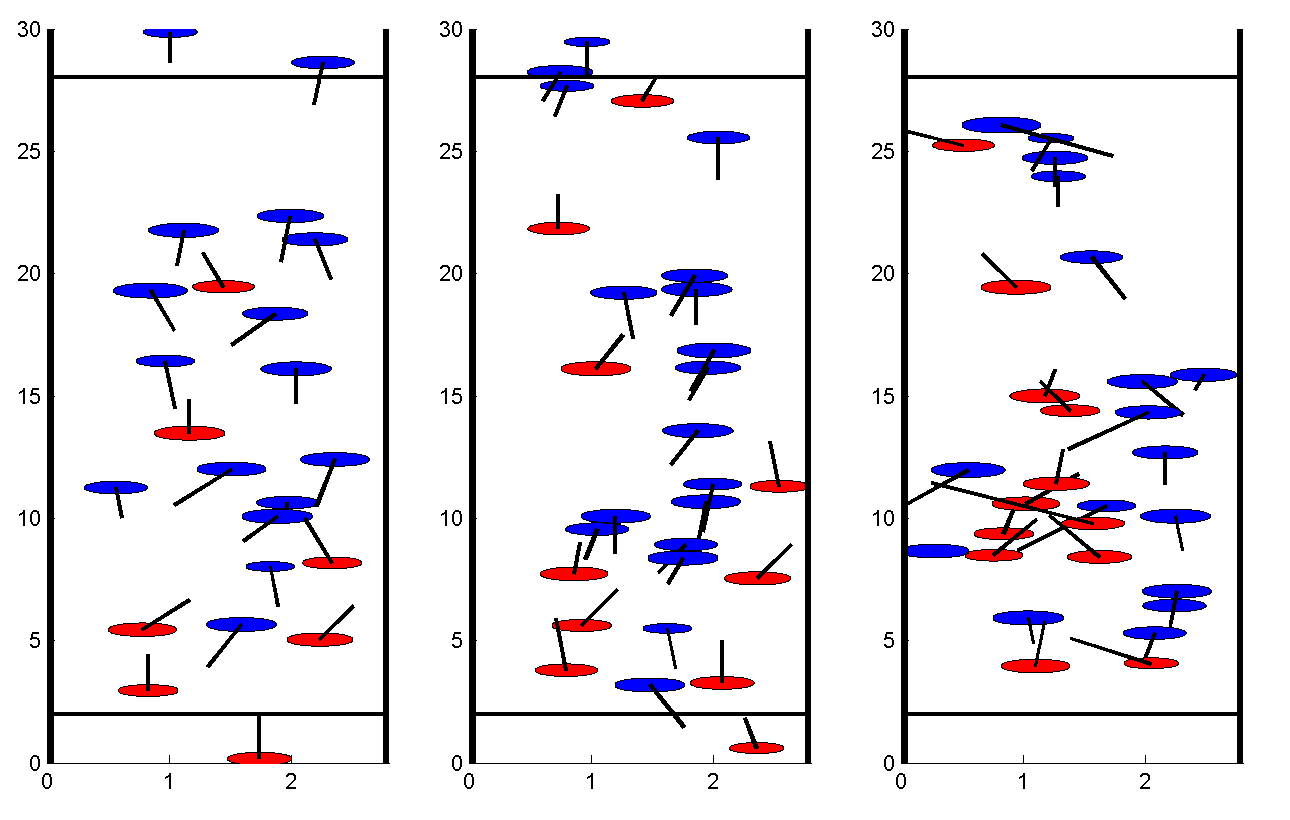
\includegraphics[width=0.90\textwidth]{pictures/ex6picture.png}
	\caption{Exemplary pictures for the simulation of the long narrow hallway in the Zurich main station with highly unbalanced flux densities. Red agents are walking up and blue down, the black line denotes the actual velocity vector with its angle and length. The one on the left was done with flux densities of 1.0/0.2, the one in the middle with 1.0/0.3 and the one on the right with 1.0/0.4 after a simulation time of 180 seconds. The red agents (minority) were wandering about quite strong and usually formed small lanes.}
	\label{fig:ex6picture}
\end{figure}

\noi For the densities 0.2/1 used in the first series, the overall success was satisfying. The agents walking up (red, minority) were wandering about quite strong due to all the oncoming blue agents. But even though the blue outnumbered the red agents 1:4, the red agents stopped very rarely.\\

\noi In the case of the densities being 0.3/1, the results were quite similar with those obtained by 0.2/1. But the tendency for the red agents to walk in lanes or small groups increased clearly, probably because there are more red agents which are shuffled together by the big number of blue agents trying to stomp their way through.\\

\noi For the last considered case, the simulation failed in one case after approximatly 140 seconds (seed 51). The situation after 180 seconds is given in figure \ref{fig:up1down03seed51} as a classical example of how a jam looks like in our model. Before that and in the other two simulations, the red agents formed lanes and little groups very frequently as a way to not always get tossed over the whole width.\\
But the failure suggests that we reached about the limit which can be modelled with our simulation.\\

\begin{figure}[h!]
	\centering
		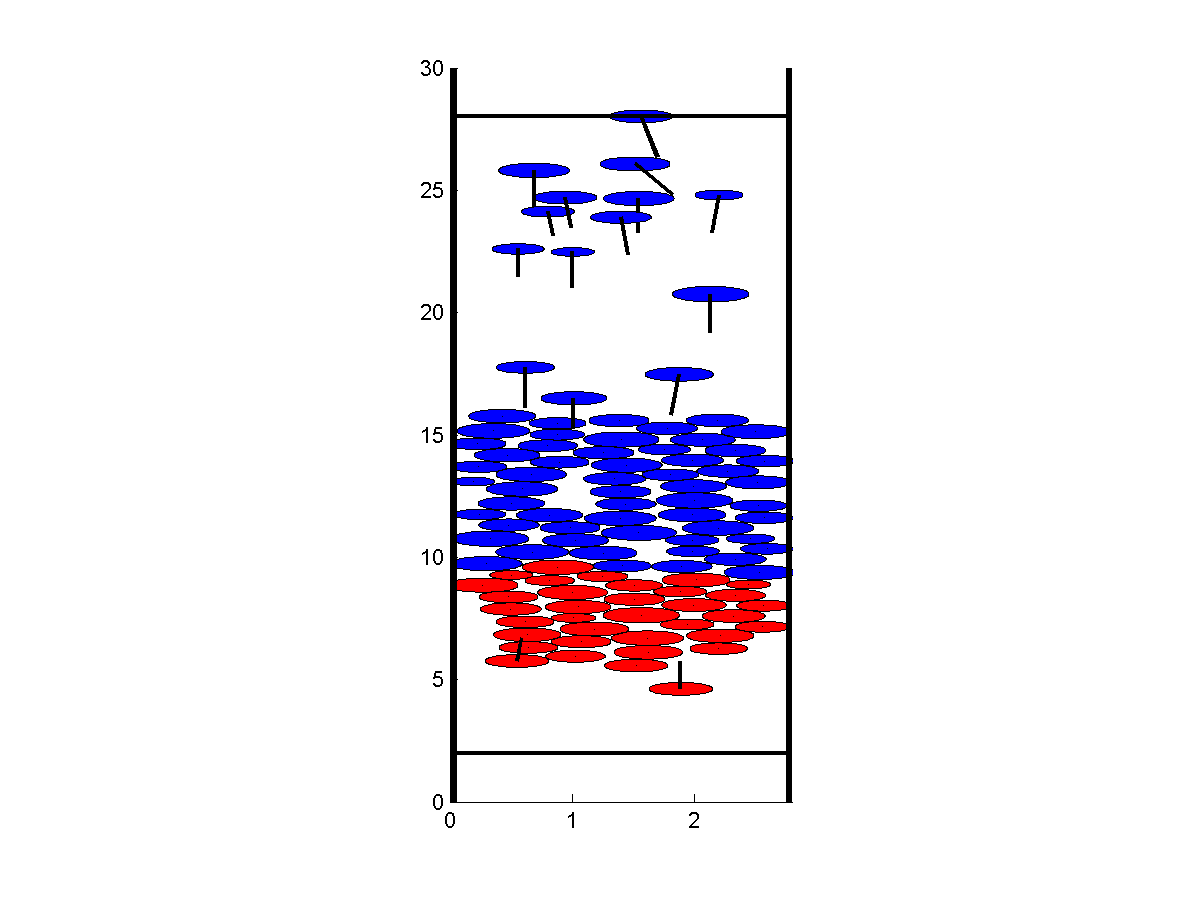
\includegraphics[width=0.90\textwidth]{pictures/up1down04seed51.png}
	\caption{Exemplary pictures for a massive jam in our model. Red agents are trying walking up and blue down, the black line denotes the actual velocity vector with its angle and length. Parameters were flux densities 0.4/1 with a seed of 51. Our model has no way to resolve a jam like that.}
	\label{fig:up1down03seed51}
\end{figure}

\noi To sum up, we can say that what we expected could be observed. Anyone who ever went against the tide, for example when people debark a train or bus, knows that advancement is hard to reach. This effect of slowing down and flocking together with other people who try to walk the same way popped up nicely.\\